\documentclass[11pt,a4paper]{article}

%----- ENHANCED TYPOGRAPHY -----
\usepackage[utf8]{inputenc}
\usepackage[T1]{fontenc}
\usepackage{lmodern}        % clean vector font
\usepackage{microtype}      % better justification & kerning
\usepackage{palatino} 
\usepackage{braket}   
\usepackage{mathtools}  % in the preamble
\usepackage{bbm}

%----- PAGE LAYOUT -----
\usepackage{geometry}
\geometry{top=1in, bottom=1in, left=1in, right=1in}
\usepackage{setspace}
\onehalfspacing  % 1.5 line spacing

%----- FANCY HEADERS & FOOTERS -----
\usepackage{fancyhdr}
\pagestyle{fancy}
\fancyhf{}
% page number outside, header text inside

\fancyhead[LO]{\small \rightmark}
\fancyhead[RO]{\small \leftmark}
\renewcommand{\headrulewidth}{0.4pt}
\renewcommand{\footrulewidth}{0pt}

% make sections feed into \leftmark/\rightmark
\renewcommand{\sectionmark}[1]{\markboth{#1}{}}
\renewcommand{\subsectionmark}[1]{\markright{#1}}

%----- SECTION NUMBERING & TOC DEPTH -----
\setcounter{secnumdepth}{3}  % number down to \subsubsection
\setcounter{tocdepth}{2}     % show ToC down to \subsection

%----- AMS MATH & THEOREM STYLES -----
\usepackage{amsmath,amssymb,mathtools}
\usepackage{amsthm}

% definitions, examples, remarks upright
\theoremstyle{definition}
\newtheorem{definition}{Definition}[section]
\newtheorem{example}[definition]{Example}
\newtheorem{remark}[definition]{Remark}

% theorems, lemmas, corollaries italic
\theoremstyle{plain}
\newtheorem{theorem}[definition]{Theorem}
\newtheorem{lemma}[definition]{Lemma}
\newtheorem{proposition}[definition]{Proposition}
\newtheorem{corollary}[definition]{Corollary}

% unnumbered proof environment
\theoremstyle{remark}

%----- OTHER PACKAGES -----
\usepackage{graphicx}
\usepackage{tikz}
\usetikzlibrary{arrows.meta,positioning}
\usetikzlibrary{calc, matrix, decorations.pathreplacing, positioning}
\usepackage{tikz-cd}
\usepackage{hyperref}
\hypersetup{colorlinks,
linkcolor=blue, citecolor=purple, urlcolor=teal}
\usepackage{enumitem}
\setlist[itemize]{nosep, left=1.5em}
\usepackage{booktabs}
\usepackage{listings}
\lstset{
basicstyle=\ttfamily\small,
numbers=left,
numbersep=5pt,
frame=single,
breaklines=true
}
\usepackage{xcolor}
\definecolor{shade}{HTML}{F5F5F5}
\usepackage{float}
%----- CUSTOM MACROS -----
\newcommand{\F}{\mathbb{F}}
\newcommand{\code}[1]{\texttt{#1}}
\newcommand{\dist}[2]{d\bigl(#1,#2\bigr)}
\newcommand{\R}{\mathbb{R}}
\newcommand{\Z}{\mathbb{Z}}
\newcommand{\N}{\mathbb{N}} 
\newcommand{\Q}{\mathbb{Q}} 
\newcommand{\C}{\mathbb{C}}
\renewcommand{\set}[1]{\left\{ #1 \right\}}
\newcommand{\angles}[1]{\langle #1 \rangle}
\newcommand{\abs}[1]{\lvert #1 \rvert}
\newcommand{\norm}[1]{\lVert #1 \rVert}
\newcommand{\1}{\mathbbm{1}}

% \usepackage{mathtools} 
% \DeclarePairedDelimiter{\angles}{\langle}{\rangle} 
% \DeclarePairedDelimiter{\braces}{\left\{}{\right\}} 
% \DeclarePairedDelimiter{\abs}{\lvert}{\rvert} 
% \DeclarePairedDelimiter{\norm}{\lVert}{\rVert}

%----- TITLE METADATA -----
\title{\LARGE\bfseries Algebraic Topology}
\author{Georges Khater \\ \small American University of Beirut, Math 314}
\date{\today}

%===============================================
\begin{document}
\maketitle
\tableofcontents
\bigskip

\section{Bases of the Fundamental Group}

\subsection{Homotopy equivalence.}
\begin{definition}
    Let $X$ be a topological space $f, g \colon X \to Y$ then we say that $f$ is \emph{homotopic} to $g$ 
    if there is a function $H \colon X \times I \to Y$ (called a homotopy) such that 
    $$H(x, 0) = f(x), \quad H(x, 1) = g(x)$$
\end{definition}

\begin{proposition}
    Homotopy is an equivalence relation. 
\end{proposition}

\begin{lemma}[Gluing Lemma]
    Suppose that $X = A \cup B$ with $A, B$ closed and take $f_1 \colon A \to Y$, $f_2 \colon B \to Y$. 
    s.t $f_1 (x) = f_2(x)$ for all $x \in A \cap B$. Then 
    $$f_3 \colon X \to Y, \quad f_3(x) = \begin{cases}
        f_1(x) \quad &\text{if $x \in A$} \\
        f_2(x) \quad &\text{if $x \in B$}
    \end{cases}$$
    is continuous.   
\end{lemma}

\begin{proof}
    Let $C$ be a closed set in $Y$, then 
    \begin{align*}
        f_3^{-1}(C) &= f_3^{-1}(C) \cap (A \cup B) \\
        &= \left(f_3^{-1}(C) \cap A\right) \cup \left( f_3^{-1} \cap B \right) \\
        &= f_1^{-1} (C) \cup f_2^{-1}(C)   
    \end{align*}
    which is closed in $X$.
\end{proof}

\begin{example}
    Any two function into $\R^n$ (convex set, start shaped set) are homotopic.

    Indeed, take two such $f(x), g(x)$ then let 
    $$H \colon X \times Y \to \R^n, \quad H(x, t) = (1-t) f(x) + t g(x)$$
    Note: we call this \emph{the straight line homotopy}. 
\end{example}

\paragraph{Relative Homotopy}
\begin{definition}
    Let $f,  g \colon X \to Y$ with $A \subseteq X$ and $f_{|A} = g_{|A}$ then 
    we say that $f$ is homotopic to $g$ relative to $A$ if there exists a homotopy $H \colon X \times I \to Y$ between $f$ and $g$ 
    $$H(x, t) = f(x) = g(x) \quad \forall t \in I, \ \forall x \in A$$ 
\end{definition}

\begin{remark}
    Homotopy is a special kind of relative  homotopy (for $A = \varnothing$). 
\end{remark}

\begin{proposition}
    Relative homotopy is an equivalence relation.
\end{proposition}

\begin{definition}
    Let $X$ a topological space and let $x_1, x_2 \in X$ then a path in $X$ going from $x_1$ to $x_2$ is a 
    function $\gamma \colon I \to X$ s.t 
    $$\gamma (0) = x_1, \quad \gamma(1) = x_2$$
\end{definition}

\begin{definition}
    Suppose that $\gamma_1$ and $\gamma_2$ are two paths in $X$ whose start point and end point coincide, then 
    we say that $\gamma_1$ is path homotopic to $\gamma_2$ if $\gamma_1$ is homotopic to $\gamma_2$ relative to $\set{0,1}$.

    Intuitively this means that we can deform $\gamma_1$ into $\gamma_2$ without moving the endpoints.
    i.e $H \colon I \times I \to X$ s.t 
    $$H (s,t) = \begin{cases}
        \gamma_1(s) \quad &\text{if } t = 0 \\
        \gamma_2(s) \quad &\text{if } t = 1 \\
        \gamma_1(0) = \gamma_2 (0) \quad &\text{if } s = 0 \\
        \gamma_1(1) = \gamma_2(1) \quad&\text{if } s = 1
    \end{cases}$$
\end{definition}

\begin{corollary}
    Path homotopy is an equivalence relation.
\end{corollary}

\begin{definition}
    $\gamma_1, \gamma_2 \colon I \to X$ with 
    $$\gamma_1(1) = \gamma_2(0)$$
    we define the \emph{product} of these paths to be the path $\gamma_1 \cdot \gamma_2$ given by 
    $$\gamma_1 \cdot \gamma_2 (s) = \begin{cases}
        \gamma(2s) \quad &\text{if } 0 \leq s \leq 1/2 \\
        \gamma(2s - 1) \quad &\text{if } 1/2 \leq s \leq 1
    \end{cases}$$
    Note that this is continuous by the Gluing Lemma.
\end{definition}

\begin{proposition}
    Path multiplication is compatible with path homotopy; i.e if 
    $$\gamma_1 \sim \gamma_1', \quad \gamma_2 \sim \gamma_2'$$
    then 
    $$\gamma_1 \cdot \gamma_2 \sim \gamma_1' \sim \gamma_2'$$
\end{proposition}

\begin{proof}
    Let $H_1 \colon I \times I \to X$ and $H_2 \colon I \times I \to X$ be the corresponding homotopies 
    then define $H \colon I \times I \to X$ by 
    $$H(s,t) = \begin{cases}
        H_1(2s,t) \quad \text{if } 0 \leq t \leq 1/2 \\
        H_2(2s-1, t) \quad \text{if } 1/2 \leq t \leq 1
    \end{cases}$$
    We have to check that this a valid path homotopy, TODO.
\end{proof}

\subsection{The Fundamental group}
\begin{definition}
    A loop in $X$ based at $x_0$ is a path whose end points are both $x_0$.
\end{definition}

\begin{theorem}
    Take $X$ a top space and $x_0 \in X$ then the set of path homotopy equivalence classes of the loops based at $x_0$ is a group where 
    multiplication, identity and inverses are defined as such: 
    \begin{itemize}
        \item $[\gamma_1] \cdot [\gamma_2] = [\gamma_1 \cdot \gamma_2]$
        \item Identity is $[x_0]$ 
        \item Inverse of $[\gamma]$ is $[\overline{\gamma}]$ where 
        $$\overline{\gamma}(s) = \gamma(1-s)$$
    \end{itemize}
    This group is called the Fundamental group of $X$ based at $x_0$ denoted by $\pi_1(X, x_0$).
\end{theorem}

\begin{remark}
    Note that multiplication is well defined, since homotopy behaves nicely with path product.
\end{remark}

\begin{lemma}
    Let $\varphi \colon I \to I$ s.t $\varphi(0) = 0$ and $\varphi(1) = 1$. Then for any path $\gamma$ we have
    that 
    $$\gamma \varphi \sim \gamma$$
    we call $\gamma \circ \varphi$ a reparametrization of $\gamma$. 
\end{lemma}

\begin{proof}
    Let $H(s, t) = \gamma ((1-t) s + t \varphi(s))$, then clearly 
    $$H(s, 0) = \gamma(s), \quad H(s,1) = \gamma(\varphi(s))$$
    $$H(0,t) = \gamma(0), \quad \gamma(1, t) = \gamma(1)$$     
\end{proof}

\begin{proof}[Proof of the theorem]
    \mbox{}\\
    We have to show that this satisfies the axioms of groups: 
    \begin{itemize}
        \item \textbf{Associativity.} Take $\gamma_1, \ \gamma_2, \ \gamma_3 \colon I \to X$ s.t 
        $$\gamma_1 (1) = \gamma_2 (0), \quad \gamma_2(1) = \gamma_3 (0)$$
        Then we have that 
        $$(\gamma_1 \cdot \gamma_2) \cdot \gamma_3 (s) = \begin{cases}
            \gamma_1 (4s) \quad &\text{if } 0 \leq s \leq 1/4 \\
            \gamma_2 (4s - 1) \quad &\text{if } 1/4 \leq s \leq 1/2 \\
            \gamma_3 (2s - 1) \quad &\text{if } 1/2 \leq s \leq 1 
        \end{cases}$$
        and 
        $$\gamma_1 \cdot (\gamma_2 \cdot \gamma_3) (s) = \begin{cases}
            \gamma_1 (2s) \quad &\text{if } 0 \leq s \leq 1/2 \\
            \gamma_2(4s - 2) \quad &\text{if } 1/2 \le s \le 3/4 \\
            \gamma_3(4s - 3) \quad &\text{if } 3/4 \le s \le 1 
        \end{cases}$$
        We want to find $\varphi \colon I \to I$ s.t 
        $$(\gamma_1 \cdot \gamma_2) \cdot \gamma_3 (s) = \gamma_1 \cdot (\gamma_2 \cdot \gamma_3) (\varphi(s))$$
        Indeed, define 
        $$\varphi (s) = \begin{cases}
            2s \quad &\text{if } 0 \leq s \le 1/4 \\
            s + 1/4 \quad &\text{if } 1/4 \leq s \leq 1/2 \\
            1/2 s + 1/2 \quad &\text{if } 1/2 \le s \le 1
        \end{cases}$$
        Check that this is a valid reparametrization; i.e that the equality above holds.

        \item \textbf{Identity.} We will only show left-identity: right is completely analogous. Take $\gamma \colon I \to X$, let 
        $x_0 = \gamma(0)$ and $x_0 \colon I \to X$ s.t $x_0(s) = x_0$. Then 
        $$x_0 \cdot \gamma (s) = \begin{cases}
            x_0 = \gamma(0) \quad &\text{if } 0 \le s \le 1/2 \\
            \gamma(2s - 1) \quad &\text{if } 1/2 \le s \le 1
        \end{cases}$$
        Then clearly $\gamma (\varphi(s)) = x_0 \cdot \gamma (s)$ via 
        $$\varphi(s) = \begin{cases}
            0 \quad &\text{if } 0 \le s \le 1/2 \\ 
            2s - 1\quad &\text{if } 1/2 \le s \le 1
        \end{cases}$$
        Check that the reparametrization is valid.
        
        \item \textbf{Inverse.} Suppose that $\gamma \colon I \to X$ is a path, fix $\alpha \in I$. Define the path 
        $$\gamma_\alpha(s) = \gamma(\alpha s)$$
        We want to show that 
        $$\gamma \cdot \overline{\gamma} \sim \gamma(0)$$
        Let $H \colon I \times I \to X$ be 
        $$H(s,t) = \gamma_{1-t} \cdot \overline{\gamma_{1-t}} (s)$$
        Then notice that 
        $$H(s,0) = \gamma_1 \overline{\gamma_1} (s), \quad H(s, 1) = \gamma_0 \cdot \overline{\gamma_0} (s) = \gamma(0)$$
        and 
        $$H(0, t) = \gamma_{1-t} (0) = \gamma(0), \quad H(1,t) = \gamma(0)$$
        Where the last equality comes from the fact that 
        $$H(s,t) = \begin{cases}
            \gamma_{1-t} (2s) \quad &\text{if } 0 \le s \le 1/2 \\
            \overline{\gamma_{1-t}} (2s - 1) = \gamma_{1-t} (2 - 2s) = \gamma((1-t) (2-2s)) \quad &\text{if } 1/2 \le s \le 1
        \end{cases}$$

        Note that $H$ is continuous since it is clearly continuous on $[0,1/2] \times I$ and $[1/2, 1] \times I$ + Gluing lemma.
    \end{itemize}
\end{proof}

\begin{theorem}
    Let $X$ be a topological space and let $x_0, x_1 \in X$; take $\eta$ a path from $x_ 0 \to x_1$. 
    Define $\beta_\eta \colon \pi_1(X, x_1) \to \pi_1 (X, x_0)$ by 
    $$\beta_\eta [\gamma] = [\eta \cdot \gamma \cdot \overline{\eta}]$$
    Then $\beta_\eta$ is an isomorphism.
\end{theorem}

\begin{proof}
    \begin{itemize}
        \item \textbf{Well defined.} Let $[\gamma_1] = [\gamma_2]$ then 
        \begin{align*}
            [\gamma_1] = [\gamma_2] &\implies \gamma_1 \sim \gamma_2 \\
            &\implies \eta \cdot \gamma_1 \sim \eta \cdot \gamma_2 \\
            &\implies \eta \cdot \gamma_1 \cdot \overline{\eta} \sim \eta \cdot \gamma_2 \cdot \overline{\eta} \\
            &\implies [\eta \cdot \gamma_1 \cdot \overline{\eta}] = [\eta \cdot \gamma_2 \cdot \overline{\eta}]
        \end{align*}
    
        \item \textbf{Homomorphism.} 
        \begin{align*}
            \beta_\eta \left([\gamma_1] \cdot [\gamma_2]\right) &= \beta_\eta \left([\gamma_1 \cdot \gamma_2]\right) \\
            &= [\eta \cdot \gamma_1 \cdot \gamma_2 \cdot \overline{\eta}] \\
            &= [\eta \cdot \gamma_1 \cdot x_1 \cdot \gamma_2 \cdot \overline{\eta}] \\
            &= [\eta \cdot \gamma_1 \cdot \overline{\eta}] \cdot [\eta \cdot \gamma_2 \cdot \overline{\eta}] \\
            &= \beta_\eta [\gamma_1] \cdot \beta_\eta [\gamma_2]
        \end{align*}

        \item \textbf{Isomorphism.} Notice that 
        \begin{align*}
            \beta_\eta \circ \beta_{\overline{\eta}} [\gamma] &= [\beta_\eta (\overline{\eta}) \cdot \gamma \cdot \eta] \\
            &= [\eta \cdot \overline{\eta} \cdot \gamma \cdot \eta \cdot \overline{\eta}] \\
            &= [x_0 \cdot \eta \cdot x_0] \\
            &= [\gamma]
        \end{align*}
        Similarly $\beta_{\overline{\eta}} \circ \beta_\eta$ is also identity.
    \end{itemize}
\end{proof}

\begin{corollary}
    If $X$ is path connected then $\pi_1(X, x_0)$ is independent of $X$.

    From now on we all space will be path connected (unless stated otherwise explicitly): in this case 
    we will simply write $\pi_1 (X)$.
\end{corollary}

\begin{definition}
    If $\pi_1(X) = e$ we say that $X$ is \emph{simply connected}
\end{definition}

\begin{proposition}
    $X$ is simply connected $\iff$ $\forall x_0, x_1 \in X$ any two paths between $x_0$ and $x$ are homotopic.
\end{proposition}

\begin{proof}
    \begin{itemize}
        \item[$\impliedby$] Take $x_0 = x_1$, then any two loops are homotopic, in particular every loop is homotopic to the constant loop.
        \item[$\implies$] Let $x_0, x_1 \in X$ and take $\gamma, \gamma' \colon x_0 \to x_1$. Note that $\gamma \cdot \overline{\gamma'}$ is a loop, 
        therefore $\gamma \cdot \overline{\gamma'} \sim x_0$. Therefore multiplying both sides by $\gamma'$ we get 
        \begin{align*}
            (\gamma \cdot \overline{\gamma'}) \cdot \gamma' &\sim x_0 \cdot \gamma' \\
            (\gamma \cdot \overline{\gamma'}) &\sim \gamma'\\
            \gamma \sim \gamma'
        \end{align*}
    \end{itemize}
\end{proof}

\begin{example}
    The following spaces are simply connected 
    \begin{itemize}
        \item $\R^n$: Let $\gamma$ be a loop based at $0$, then let 
        $$H(s, t) = (1-t) \gamma(s) + t \cdot x_0 = (1-t) \gamma(s)$$
        \item Similarly, every convex set is simply connected. 
        \item Similarly, every star-shaped set is simply connected. 
        \item $S^n$ is simply connected for $n \geq 2$ (proof later).
    \end{itemize}
    Notice that $S^1$ is not simply connected (proof later).
\end{example}

\subsection{Homotopy of spaces}
Let $X, Y$ be topological spaces and $\varphi \colon X \to Y$ be a map. Fix $x_0 \in X$, suppose that 
$\gamma$ is a loop based at $x_0$, then $\varphi (\gamma)$ is a loop based at $\varphi(x_0)$. 
Moreover, if $\gamma \sim \gamma'$ via homotopy $H$, then $\varphi (\gamma) \sim \varphi(\gamma')$ via the homotopy
$\varphi \circ H$. 

\begin{proof}
    $H \colon I \times I \to X$ s.t 
    $$H(0, t) = x_0 = H(1, t), \quad H(s, 0) = \gamma(s), \quad H(s, 1) = \gamma'(s)$$
    Then 
    $$\varphi \circ H \colon I \times I \to Y$$
    and 
    $$\varphi(H(0,t)) = \varphi(x_0) = \varphi (H(1, t)), \quad H(s,0) = \varphi(\gamma(s)) , \quad \varphi(H(s,1)) = \varphi(\gamma'(s))$$
\end{proof}

Therefore we get a well defined map from $\pi(X, x_0)$ to $\pi(Y, \varphi(x_0))$, denote by 
$\varphi_*$ and defined by 
$$\varphi_* ([\gamma]) = [\varphi \circ \gamma]$$

\begin{proposition}
    \begin{itemize}
        \item $\varphi_*$ is a Homomorphism. 
        \item $(\psi \circ \varphi)_* = \psi_* \circ \varphi_*$. 
        \item $(\mathbbm{1})_* = \mathbbm{1}_*$
        \item $\varphi \sim \psi$ relative to $x_0$ then $\varphi_* = \psi_*$.  
    \end{itemize}
\end{proposition}

\begin{proof}
    \begin{itemize}
        \item Take $\gamma_1, \gamma_2$ loops at $x_0$, then 
        \begin{align*}
            \varphi(\gamma_1 \cdot \gamma_2) = \varphi(\gamma_1) \cdot \varphi(\gamma_2)
        \end{align*}
        because 
        $$\varphi(\gamma_1 \cdot \gamma_2 (s)) = \begin{cases}
            \varphi(\gamma_1 (2s)) \quad 0 \le s \le 1/2 \\
            \varphi(\gamma_2 (2s-1)) \quad 1/2 \le s \le 1
        \end{cases}$$
        but 
        $$\varphi(\gamma_1) \cdot \varphi(\gamma_2) (s) = \begin{cases}
            \varphi(\gamma_1(2s)) \quad 0 \le s \le 1/2 \\
            \varphi(\gamma_2(2s-1) \quad 1/2 \le s \le 1)
        \end{cases}$$
        Therefore 
        \begin{align*}
            \varphi_*([\gamma_1] \cdot [\gamma_2]) &= \varphi_*([\gamma_1 \cdot \gamma_2]) \\
            &= [\varphi(\gamma_1 \cdot \gamma_2)] = [\varphi(\gamma_1) \cdot \varphi(\gamma_2)] \\
            &= [\varphi(\gamma_1)] \cdot [\varphi(\gamma_2)] \\
            &= \varphi_*([\gamma_1]) \cdot \varphi_*([\gamma_2])
        \end{align*}
        \item TODO 
        \item TODO 
        \item Let $\gamma$ be a loop at $x_0$ and suppose that $H$ is the homotopy between $\varphi$ and $\psi$ relative to $x_0$, therefore 
        $H \colon X \times I \to Y$ s.t 
        $$H(x, 0) = \varphi(x), \quad H(x, 1) = \psi(x), \quad H(x_0, t) = \varphi(x_0) = \psi(x_0)$$
        Then consider the map 
        $$H' \colon I \times I \to Y, \quad H'(s, t) = H(\gamma(s), t)$$
        then 
        $$H'(s, 0) = H(\gamma(s), 0) = \varphi(\gamma(s)), \quad H'(s, 1) = H(\gamma(s), 1) = \psi(\gamma(s))$$
        and 
        $$H'(0, t) = H(x_0, t) = \varphi(x_0), \quad H'(1,t) = \psi(x_0)$$
        Therefore for any $\gamma$ 
        $$\varphi_*([\gamma]) = [\varphi(\gamma)] = [\psi(\gamma)] = \psi_*([\gamma])$$
    \end{itemize}
    draw the pictures here, it clears things up. 
\end{proof}

\begin{corollary}
    $X \cong Y \implies \pi_1(X) \cong \pi_1 (Y)$. 
\end{corollary}

\begin{proof}
    Let $\varphi \colon X \to Y, \quad \psi \colon Y \to X$  such that 
    $$\psi \circ \varphi = \mathbbm{1}_{X}, \quad \varphi \circ \psi = \mathbbm{1}_Y$$
    Therefore 
    $$(\psi \circ \varphi)_* = \psi_* \circ \varphi_* = \mathbbm{1}_*$$
    similarly 
    $$\varphi_* \circ \psi_* = \mathbbm{1}_*$$
    Therefore 
    $$\pi_1(X) \cong \pi_1(Y)$$
\end{proof}

\begin{remark}
    Note that the proof above would still work if we only had that $\psi \circ \varphi \sim \mathbbm{1}$ relative to $x_0$ and 
    $\varphi \circ \psi \sim \mathbbm{1}$ relative to $\varphi(x_0)$.
\end{remark}

\begin{definition}
    Let $X, Y$ be two spaces, we say that $X$ is \emph{homotopic} to $Y$ iff there exists some 
    $\varphi \colon X \to Y$ and $\psi \colon Y \to X$ such that 
    $$\psi \circ \varphi \sim \mathbbm{1}_X, \quad \varphi \circ \psi \mathbbm{1}_Y$$
\end{definition}

\begin{proposition}
    Homotopy of spaces is an equivalence relation
\end{proposition}

\begin{proof}
    \begin{itemize}
        \item \textbf{Reflexive.} Take $\varphi = \psi = \mathbbm{1}$. 
        \item \textbf{Symmetric.} Trivial. 
        \item \textbf{Transitive.} \begin{lemma}
            Let $f \colon X \to Y$, $f' \colon X \to Y$ $g, g' \colon Y \to Z$ with 
            $$f \sim f', \quad g \sim g'$$
            then 
            $$g \circ f \sim g' \circ f'$$
        \end{lemma}
        \begin{proof}
            Let $H$ be the homotopy between $f$ and $f'$ and $H'$ is the homotopy between $g$ and $g'$. Then 
            $$H'' \colon X \times I \to Z$$
            defined by 
            $$H''(x, t) = H'(H(x, t) ,t)$$ 
            notice that 
            $$H''(0, t) = H'(H(x,0), 0) = H'(f(x), 0) = g \circ f (x)$$
            Similarly check the rest. 
        \end{proof}
        Now suppose we have $X, Y, Z$ spaces with 
        $$\varphi \colon X \to Y, \quad \varphi \colon Y \to \Z$$ 
        and 
        $$\psi \colon Y \to X, \quad \psi' Y \to Z$$ 
        \[
        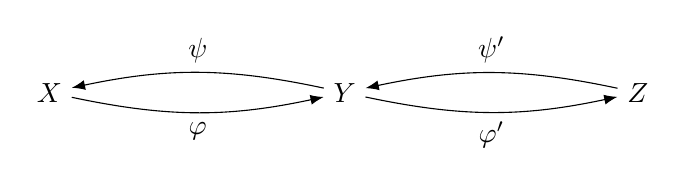
\begin{tikzpicture}[>=Latex, node distance=3.2cm]
        \node (X) {$X$};
        \node (Y) [right=of X] {$Y$};
        \node (Z) [right=of Y] {$Z$};

        % forward maps
        \draw[->] (X) to[bend right=12] node[below] {$\varphi$} (Y);
        \draw[->] (Y) to[bend right=12] node[below] {$\varphi'$} (Z);

        % backward maps (drawn slightly below)
        \draw[->] (Y) to[bend right=12] node[above] {$\psi$} (X);
        \draw[->] (Z) to[bend right=12] node[above] {$\psi'$} (Y);
        \end{tikzpicture}
        \]
        Then 
        $$\varphi' \circ \varphi \colon X \to Z, \quad \psi \circ \psi' \colon Z \to X$$
        s.t 
        \begin{align*}
            \psi \circ \psi' \circ \varphi' \circ \varphi &\sim \psi \circ \mathbbm{1} \circ \varphi \\
            &\sim \mathbbm{1}
        \end{align*}
    \end{itemize}
\end{proof}

\paragraph{Terminology.} If $X \sim \set{\cdot}$, then we say that $X$ is contractible. 
\begin{example}
    $\R^n$ is contractible; there is only one map $\varphi \colon \R^n \to \set{\cdot}$. Take the map $\psi \colon \cdot \to \R^n$ to be
    $$\cdot \to 0$$
    Indeed 
    $$\varphi \circ \psi \colon \cdot \to \cdot = \1$$

    Moreover, $\psi \circ \varphi \colon \R^n \to \R^n$ 
    $$\psi \circ \varphi (\alpha) = 0$$
    let $H \colon \R^n \times i \to \R^n$ defined by 
    $$H(x, t) = t \cdot x$$
    Similarly, we get that any convex subset of $\R^n$ is contractible; any star-shaped set is also contractible.

    Later on we will see that $S^n$ is not contractible. 
\end{example}

\begin{definition}
    Let $X$ be a space and $A \subseteq X$, then $r \colon X \to A$ is called a \emph{retraction} iff 
    $$r_{|A} = \1_{|A}$$
    In this case we say that $A$ is a \emph{retract} of $X$.
\end{definition}


\begin{example}
    \begin{itemize}
        \item Clearly the function $r \colon \R^n \to \set{x_0}$ is a retraction.
        \item $r \colon \R^n \setminus \set{0} \to S^{n-1}, \quad x \to \frac{x}{|x|}$
    \end{itemize}
\end{example}

\begin{definition}
    $X$ a space, $A \subseteq X$: we say that $X$ deformation retracts to $A$ (or that there is a deformation retraction from $x$ to $A$) 
    (or that $A$ is a deformation retract of $X$) iff 
    \begin{itemize}
        \item There is a retraction $r \colon X \to A$. 
        \item Letting $\iota \colon A \to X$ be the inclusion map, we have 
        $$r \circ \iota = \1_{|A}$$
        and 
        $$\iota \circ r \sim \1_{|A} \text{ relative to $A$}$$
    \end{itemize}
\end{definition}

\begin{example}
    \begin{itemize}
        \item $\R^n$, convex / start shaped subsets deformation retract into a point. 
        \item $\R^n$ deformation retract into $D^n$: let $r \colon \R^n \to D^n$ be defined by 
        $$r(x) = \begin{cases}
            x \quad &\text{if } x \in D^n \\
            \frac{x}{|x|} \quad &\text{if } x \not\in D^n
        \end{cases}$$
        Let $H(x, t) = t r(x) + (1-t)x$. 
        \item $\R^n \setminus \set{0}$ deformation retracts to $S^{n-1}$: $r \colon \R^n \setminus \set{0} \to S^{n-1}$ by 
        $$r(x)  = \frac{x}{|x|}$$
        $H(x,t) = (1-t) x + t \frac{x}{|x|}$ is the homotopy. 

        There is no deformation retraction from $\R^n \setminus \set{0}$ to any point.

        \item $I \times I$ (The closed rectangle) deformation retracts to a cup Exercise. 
    \end{itemize}
\end{example}

\begin{proposition}
    If $X$ deformation retracts to $A$ and $A$ to $B$, then $X$ deformation retracts to $B$.
\end{proposition}

\begin{proof}
    Exercise.
\end{proof}

\begin{theorem}
    $X \sim Y \implies \pi_1(X) \cong \pi_1(Y)$ 
\end{theorem}

\begin{lemma}
    Let $X, Y$ topological spaces and $\varphi, \psi \colon X \to Y$ be two homotopic functions by a homotopy $H \colon X \times I \to Y$. 
    Note that $H(x_0, \cdot)$ is a path in $Y$ (denote it by $\eta$). Then the following diagram commutes:
    \[
    \begin{tikzcd}
    \pi_1(X,x_0) \arrow[r,"\psi_*"] \arrow[dr,swap,"\varphi_*"] &
    \pi_1\bigl(Y,\psi(x_0)\bigr) \arrow[d,"\beta_\eta"] \\
    & \pi_1\bigl(Y,\varphi(x_0)\bigr) 
    \end{tikzcd}
    \]
    i.e 
    $$\beta_\eta \circ \psi_* = \varphi_*$$ 
\end{lemma}

\begin{proof}[Proof of lemma]
    Let $\gamma \colon I \to X$ be a loop based at $x_0$, let 
    $$H'(s,t) = \eta_t (s) \cdot H(\gamma(s), t) \cdot \overline{\eta_t} (s)$$
    Convince yourself that the endpoints match here; therefore by the Gluing Lemma $H'$ is continuous. 
    \begin{itemize}
        \item At $t = 1$, we get 
        $$\eta \cdot \psi (\gamma) \cdot \overline{\eta}$$
        \item At $t = 0$, we get 
        $$\varphi(x_0) \cdot \varphi(\gamma) \cdot \overline{\varphi(x_0)}$$
    \end{itemize}
    So we have that 
    \begin{align*}
        \eta \cdot \psi (\gamma) \cdot \overline{\eta} &\sim \varphi(x_0) \cdot \varphi(\gamma) \overline{\varphi} (x_0) \\
        &\sim \varphi (\gamma)
    \end{align*} 
    and therefore
    \begin{align*}
        [\eta \cdot \psi (\gamma) \cdot \overline{\eta}] &= [\varphi (\gamma)]  \\
        \beta_\eta [\psi(\gamma)] &= \varphi_* ([\gamma]) \\
        \beta_\eta(\psi_*([\gamma])) &= \varphi_* ([\gamma])
    \end{align*}
    therefore 
    $$\varphi_* = \beta_\eta \circ \psi_*$$
\end{proof}

\begin{proof}[Proof of the theorem]
        \[
    \begin{tikzcd}[column sep=huge]
    (Y,y_0) \arrow[r,"\psi"] &
    (X,x_0) \arrow[r,"\varphi"] &
    (Y,y_1) \arrow[r,"\psi"] &
    (X,x_1)
    \end{tikzcd}
    \]
    we know that 
    $$\psi \circ \varphi \sim \1, \quad \varphi \circ \psi \sim \1$$
    Therefore by the lemma 
    $$(\psi \circ \varphi)_* = \beta, \quad (\varphi \circ \psi)_* = \beta'$$
    But $\beta, \beta'$ are isomorphisms, therefore we get that 
    $$\varphi_* \text{ is injective and surjective}$$
\end{proof}

\subsection{Fundamental group of all spheres} 

\begin{theorem}
    $$\pi_1(S^n) = \begin{cases}
       e \quad &\text{if } n \ge 2 \\
       \Z \quad &\text{if } n = 1 \\ 
    \end{cases}$$
\end{theorem}

\begin{proof}
    \begin{itemize}
        \item $\pi_1(S^2)$; there is a homeomorphism between $S^2 \setminus \set{N}$ and $\R^2$ ($N$ is the North pole) called the stereographic projection. 
        i.e $t \to (0,0,1) + t(x, y,z) = (tx,ty, tx + 1)$ since $1 + tz = 0 \implies t = \frac{t}{1-z}$ we get the map $\Sigma$ given by 
        $$\Sigma (x,y,z) = (\frac{x}{1-z}, \frac{y}{1-z})$$
        For the inverse map $t \to (0,0,1) + t(\alpha, \beta, -1) = (t \alpha, t \beta, 1 - t)$; on the sphere 
        $$t^2 \alpha^2 + t^2 \beta^2 + (1-t)^2 = 1 \implies t = \frac{2}{\alpha^2 + \beta^2 + 1}$$
        so its inverse is given by 
        $$\Sigma^{-1} (\frac{2}{\alpha^2 + \beta^2 + 1}, \frac{2 \beta}{\alpha^2 + \beta^2 + 1}, 1 - \frac{2}{\alpha^2 + \beta^2 + 1})$$
        TODO, do the same for $\R^n$. 

        We shall take our loops to be based at the south pole $S$. Let $\gamma \colon I \to S^2$ be such a loop. If it happens that $\gamma$ never passes through $N$; 
        $\Sigma \circ \gamma$ is a loop in $\R^2$ based at $0$. Thus $H \colon I \times I \to S^2$ given by 
        $$H(s, t) = \Sigma^{-1}\left((1-t) \Sigma \circ \gamma (s) \right)$$
        gives a homotopy between $\gamma$ and the constant loop at the south pole. 

        Now suppose that we have any loop $\gamma \colon I \to S^2$. Consider the preimage by $\gamma$ of the open Northern hemisphere, this is 
        open in $I$ since $\gamma$ is continuous; in fact it is open in $(0,1)$ (and hence an open subset of $\R$). Now any open subset of $\R$ is the union of countably many 
        disjoint open intervals. Consider now the preimage of $N$, it must be closed in $[0,1]$ and hence must be compact. Therefore since the preimage of the open Northern hemisphere 
        contains that of $N$; the preimage of $N$ is an open cover of the preimage of $N$. So it has a finite subcover. Thus there are finitely many disjoint open intervals which 
        contain the preimage of $N$. Consider one of these intervals $(a, b)$. Note that $\gamma((a,b)) \subseteq N$; since $\gamma$ is continuous we can conclude that 
        $\gamma(a), \gamma(b) \in \overline{N}$ (the closed Northern hemisphere). Note that $\gamma(a), \gamma(b)$ must be on the equator; since if they were in the Northern hemisphere we would have that 
        $a$ belongs to one of the other \emph{disjoint} intervals to $(a, b)$. Note that the closed Northern hemisphere is homeomorphic to $D^2$ by $(x, y, z) \to (x,y)$. 
        but note that $\partial D^2 = S^1$ which is path connected; since we can find some path $\eta \colon I \to S^1$ going from $\gamma(a) \to \gamma(b)$ with $\eta$ homotopic $\gamma_{|[a,b]}$. 

        Now we can write a homotopy between $\gamma$ and some loop that skips $N$; see the picture we are using the homotopy above on all $(a,b)$ like above. This is continuous by the gluing 
        lemma according to our homotopy. So $\gamma$ is homotopic to a loop that skips $N$ and so homotopic to the constant loop. 

        \item We will think of $S^1$ as 
        $$\set{z \in \C \colon |z| = 1}$$
        We will base our loops at the point $z = 1$. We define 
        $$\Phi \colon \Z \to \pi_1(S^1), \quad \Phi (n) = [e^{2 \pi i n s}]$$
        We also define 
        $$p \colon \R \to S^1, \quad p(x) = e^{2 \pi i x}$$
        Note that $[p(ns)] = \Phi(n)$. We will show that $\Phi$ is a homomorphism
        \begin{align*}
            \Phi(n) \cdot \Phi(m) &= [p(ns)] \cdot [p(ms)] \\
            &= [p(ns) \cdot p(ms)] \\
            &= [p(ns) \cdot p(n + ms)] \\
            &= [p(ns \cdot (n + ms))] \\
        \end{align*}
        Note that $ns \cdot (n + ms)$ is a path $0 \to m + n$, but $\R$ is simply connected, hence 
        $$ns \cdot (n + ms) \sim (n + m)s \implies p(ns \cdot (n + ms)) \sim p((n+m) \cdot s)$$
        Therefore 
        $$\Phi(n) \cdot \Phi(m) = [p(n+m)s] = \Phi(n+m)$$
        \textbf{Claim 1.} For any path $\gamma$ in $S^1$ starting at $1$, there is a unique path $\tilde{\gamma} \in \R$ starting at $0$, s.t 
        $$p(\tilde{\gamma}) = \gamma$$
        we say that $\tilde{\gamma}$ is the \emph{lift} of $\gamma$ starting at $0$. \\
        \textbf{Claim 2.} Suppose that $\gamma_1, \gamma_2$ are two paths in $S^1$ starting at $1$, which are homotopic. Then their lifts starting at $0$ 
        are also homotopic. \\
        \textbf{$\Phi$ is surjective.} Let $[\gamma] \in \pi_1(S^1)$, then we know that there is a unique $\tilde{\gamma}$ in $\R$ s.t 
        $$\tilde{\gamma} (0) = 0, \quad p(\tilde{\gamma}) = \gamma$$
        Especially $p(\tilde\gamma(1)) = \gamma(1) = 1$, hence 
        $$\tilde \gamma(1) = n \in \Z \implies \tilde \gamma \sim ns$$
        Therefore 
        $$p(\tilde \gamma) \sim p (ns) \implies \gamma \sim p(ns) \implies [\gamma] = [p(ns)] = \Phi(n)$$
        \textbf{$\Phi$ is injective.} Suppose that $\Phi(n) = \Phi(m)$ therefore 
        $$[p(ns)] = [p(ms)]$$
        We have that the lift of $p(ns)$ is $ns$ and the lift of $p(ms)$ is $ms$ but 
        $$p(ns) \sim p(ms) \implies ns \sim ms \implies n = m$$

        We will prove the two claims in the following setting: $\tilde X, X$ two spaces, $p \colon \tilde X \to X$ s.t 
        $\forall p \in X, \ \exists U \ni p$ open then $p^{-1}(U)$ is a disjoint union of open sets s.t each one of them (say $V$) satisfies 
        $$p_{|V} \quad \text{ is a homeomorphism onto $U$}$$
        Such a $U$ is called an elementary neighborhood or an evenly covered neighborhood. $p$ is called the projection covering map and 
        $$(\tilde X, p) \text{ is called a covering space of } X$$
        The example to take in mind here is $X = S^1$, $\tilde X = \R$ with $p$ "wrapping" $\R$ around $S^1$. Indeed consider $U_1 = S^1 \setminus \set{1}$, then 
        $p^{-1} (U_1)$ $\R \setminus \Z$;  and $U_2 = S^1 \smallsetminus \set{-1}$ then $p^{-1} (U_2)$ and $U_2 = \R \setminus (1/2 \Z)$, so $(\R, p)$ is indeed a covering space 
        of $S^1$.\\
        \textbf{Claim 3.} Suppose that $(\tilde X, p)$ is a covering space of $X$, and let $f \colon Y \times I \to X$ and suppose we have some $\tilde f \colon Y \times \set{0} \to \tilde X$ 
        s.t 
        $$p \circ \tilde f = f$$
        then $\tilde f$ can be extended \emph{uniquely} to $Y \times I$ s.t $p \circ \tilde f = f$ (draw the picture).  \\
        \textbf{Proof that claim 3 implies claim 1 and 2.} For claim 1, let $Y = \set{\cdot}$, in this case 
        $$\set{\cdot} \times I \cong I$$
        so we have that $f \colon I \to X$ and $\tilde f \colon 0 \to \tilde X$ s.t $\tilde f$ can be uniquely extended to $I$; which is precisely claim 1
        where we are given a path in $X$ and the starting point of the lift is $\tilde X$. For claim 2, take $Y = I$ and $f$ to be the homotopy between 
        the two paths in $X$; from claim 1 we can lift the homotopy at the initial time; claim 3 lifts the homotopy to $\tilde X$. By uniqueness of lifts 
        the sides of the homotopy lift to the constant paths and the top of the homotopy gives a lift of the second path starting where the lift of the first path started.   

        \textbf{Proof of claim 3.} Let $y \in Y$, $\forall t \in I$ there is an open neighborhood $O_t$ of $t$ in $I$ and an open neighborhood $N_t$ of $y$ in $Y$ s.t 
        $$f(N_t \times O_t) \subseteq \text{ an elementary neighborhood}$$ 
        $\set{y} \times I$ is compact and $\set{N_t \times O_t}_{t \in I}$ is an open cover, therefore $\exists t_1, \cdots, t_k \in I$ s.t
        $$\set{y} \times I \subseteq (N_{t_1} \times O_{t_1}) \cup \cdots \cup (N_{t_k} \times O_{t_k})$$
        Let $N = \bigcap_{i = 1}^k N_{t_i}$, and let $\delta > 0$ be the Lebesgue number of the cover $O_{t_1}, \cdots, O_{t_k}$. Therefore any closed interval of length 
        $\le \delta$ is contained in one of the $O_t$'s. Consider $N \times [0, \delta]$ we know that $f (N \times [0, \delta]) \subset U$ an elementary neighborhood.
        But $p \circ \tilde f = f$, therefore $\tilde f (N \times {0}) \subset p^{-1} (U)$, let $\tilde U$ be the "part" of $p^{-1} (U)$ which contains $\tilde f (y,0)$. Now by taking the preimage 
        of $\tilde U$ by $\tilde f$ we get some open subset of $Y$ which is also an open subset of $N$; replace $N$ with this smaller subset call it $N$. Now $p$ is a homeomorphism between 
        $\tilde U$ and $U$, so it has an inverse $p^{-1} \colon U \to \tilde U$, define 
        $$\tilde f = p^{-1} \circ f$$
        This way, we have extended $\tilde f$ to $N \times [0, \delta]$. Now do the same for $N \times [\delta, 2\delta]$ by looking at $\tilde f (N \times \set{\delta})$ and making sure that 
        it maps to only one of the preimages of the new elementary neighborhood, we shrink $N$ again and extend $\tilde f$ by letting it be $p^{-1} \circ f$.   
        
        Note that by construction we have that $p \circ \tilde f = f$, and it is continuous by the Gluing lemma. Hence we know that $\forall y \in Y$, $\exists N_y$ s.t 
        $\tilde f$ is extended continuously to include $N_y \times I$ with $p \circ \tilde f = f$. Let us show that lifts of paths are unique; indeed suppose that we 
        have $\gamma \colon I \to X$ a path in $X$, and let $\tilde \gamma_1, \ \tilde \gamma_2$ be two lifts of $\gamma$ (i.e $p \circ \tilde \gamma_1 = p \tilde \gamma_2 = \gamma$ and they both have the same start point). 
        Therefore $\exists \delta > 0$ s.t any closed interval of length $\delta$ is mapped by $\gamma$ into an elementary neighborhood. Consider the interval $[0, \delta]$, we know that 
        $$\gamma \left([0,\delta]\right) \subset \text{ an elementary neighborhood $U$}$$ 
        This implies that $\tilde \gamma_1 ([0,\delta]) \subset p^{-1}(U)$ and $\tilde \gamma_2 ([0, \delta]) \subset p^{-1} (U)$; since $[0,\delta]$ is connected, we know that 
        $$\gamma_1 ([0,\delta]), \ \gamma_2 ([0,\delta]) \subset \text{ a single $\tilde U_1, \tilde U_2$}$$
        since $\tilde \gamma_1 (0) = \tilde \gamma_2 (0)$ we get $\tilde U_1 = \tilde U_2$. But since $p \circ \tilde \gamma_1 = p \circ \tilde \gamma_2$ and 
        since $p$ is a homeomorphism, then 
        $$\tilde U_1 = \tilde U_2 \to 0$$
        Proceeding similarly, we get that $\tilde \gamma_1 = \tilde \gamma_2$. 

        Note that restricting $f$ to a line like $\set{y} \times I$ gives a path in $X$, and restricting $\tilde f$ to this line gives us a lift of this path. So if we use $\tilde f$'s coming
        from different $N_y \times I$'s, then they must coincide on the intersection because the intersection is made of lines as above. So $\tilde f$ and $\tilde f$ is unique. And $\tilde f$ is continuous 
        using the gluing lemma for open sets. 
    \end{itemize}
\end{proof}

\begin{theorem}[Fundamental theorem of Algebra]
    Let $p(z) = z^n + a_{n-1} z^{n-1} + \cdots + a_0$ then 
    $$p(z_0) = 0 \text{ for some $z_0 \in \C$}$$     
\end{theorem}

\begin{proof}
    Assume that $p(z) \ne 0$ consider 
    $$H_1(s, t) = \frac{\frac{p(tre^{2 \pi i s})}{|p(tre^{2\pi i s|})}}{\frac{p(tr)}{|p(tr)|}}$$
    Note that this gives a homotopy between the constant loop  in $S^1$ at $1$ and $\frac{\frac{p(re^{2\pi i s})}{|p(re^{2 \pi i s})|}}{\frac{p(r)}{|r|}}$. Choose $r > 0$ 
    to be s.t $r > 1$ and $r > |a_{n-1}| + \cdots + |a_0|$, then notice that if $z$ is restricted to the circle of radius $r$, we have that 
    \begin{align*}
        |z|^n &= r^n = r^{n-1} \cdot r > r^{n-1} (|a_{n-1}| + \cdots + |a_0|) \\
        &> r^{n-1} |a_{n-1}| + \cdots + r^{n-1} |a_0| \\
        &> r^{n-1} |a_{n-1}| + r^{n-2} |a_{n-2}| + \cdots + |a_0| \\
        &= |a_{n-1} z^{n-1}| + \cdots + |a_0| \\
        &\ge |a_{n-1} z^{n-1} + \cdots + a_0|
    \end{align*} 
    it follows that the following polynomials depending on $t$ never vanish on the circle of radius $r$: 
    $$q_t(z) = z^n + t(a_{n-1} z^{n-1} + \cdots + a_0)$$
    This is because for $|z| = r$ we have that 
    $$q_t(z) \ge |z^n| - |t(a_{n-1} z^{n-1} + \cdots + a_0)| > 0$$
    Now consider $H_2(s,t)$ to be 
    $$H_2(s, t) = \frac{\frac{q_t(re^{2 \pi i s})}{|q_t(re^{2\pi i s|})}}{\frac{q_t(r)}{|p(r)|}}$$
    Note that this gives a homotopy between the loop which we just created (write it out TODO); and 
    $$\frac{\frac{r^n e^{2 \pi i n s}}{r^n}}{r^n/r^n} = e^{2 \pi n s}$$
    Therefore using both $H_1$ and $H_2$ we have a homotopy between the constant loop and $e^{2 \pi i ns}$ by contradiction. 
\end{proof}

\begin{theorem}[Brouwer's fixed point]
    $f \colon D^n \to D^n$ then $f$ has a fixed point, i.e $\exists p_0 \in D^n$ s.t 
    $$f(p_0) = p_0$$    
\end{theorem}




\end{document}